\documentclass[cic,tc,english]{infufrgs}

\usepackage[utf8]{inputenc}
\usepackage{graphicx}
\usepackage{subcaption}
\usepackage{float}
\usepackage{algorithm}
\usepackage{algpseudocode}
\usepackage{xcolor}
\usepackage{listings}
\usepackage{hyperref}
\usepackage{glossaries}

\renewcommand{\glstextformat}[1]{#1}
\makeglossaries
\newglossaryentry{dynamic partitioning}
{
  name=dynamic partitioning,
  description={A type of partitioning in which the segmentation of
    the domain varies throughout the application's lifetime, increasing or
    decreasing the amount of computation handled by the workers as the
  execution moves forward}
}
\newglossaryentry{worker}
{
  name=worker,
  description={A process in the topology responsible for
  one or more chunks of computational jobs}
}
\newglossaryentry{sample}
{
  name=sample,
  description={The smallest computational unit to be processed}
}
\newglossaryentry{halo}
{
  name=halo,
  description={The region on the outskirts of a process's
    computational grid on which
  neighboring nodes depend for their calculations}
}
\newglossaryentry{coordinator}
{
  name=coordinator,
  description={A specific process, commonly the one identified by
    rank $0$, which is often responsible for distributing work across
  all nodes and reassembling the generated data.}
}
\newacronym{vti}{VTI}{Vertical Transversal Isotropy}
\newacronym{tti}{TTI}{Tilted Transversal Isotropy}
\newacronym{oom}{OOM}{Out Of Memory}
\newacronym{fma}{FMA}{Fused Multiply-Add}
\newacronym{flop}{FLOP}{Floating-point operation}

\definecolor{mGreen}{rgb}{0,0.6,0}
\definecolor{mGray}{rgb}{0.5,0.5,0.5}
\definecolor{mPurple}{rgb}{0.58,0,0.82}
\definecolor{backgroundColour}{rgb}{0.95,0.95,0.92}

\lstdefinestyle{CStyle}{
  backgroundcolor=\color{backgroundColour},
  commentstyle=\color{mGreen},
  keywordstyle=\color{blue},
  numberstyle=\tiny\color{mGray},
  stringstyle=\color{mPurple},
  basicstyle=\ttfamily\footnotesize,
  breakatwhitespace=false,
  breaklines=true,
  captionpos=b,
  keepspaces=true,
  numbers=left,
  numbersep=5pt,
  showspaces=false,
  showstringspaces=false,
  showtabs=false,
  tabsize=2,
  language=C,
  morekeywords={MPI_Init, MPI_Finalize, MPI_Comm_rank, MPI_Comm_size,
    MPI_Send, MPI_Recv, MPI_Isend, MPI_Irecv, MPI_Waitall,
    MPI_Cart_create, MPI_Cart_shift, MPI_Comm, MPI_Dims_create,
  MPI_Cart_coords, MPI_Cart_rank}
}
\lstset{
  basicstyle=\ttfamily,
  keywordstyle=\color{blue},
  breaklines=true
}

\title{Distributed Implementation of Anisotropic RTM Using the
Fletcher Method with MPI and Ghost Cells}
\author{Spadotto}{Vinícius Daniel}
\advisor[Prof.~Dr.]{Mello Schnorr}{Lucas}
\date{March}{2026}

\keyword{RTM}
\keyword{Fletcher}
\keyword{MPI}
\keyword{Ghost Cell}
\keyword{Halo}

\begin{document}
\maketitle
\begin{abstract}
  Petroleum exploration, in the current landscape, remains the main source of
  power that fuels modern society. In such a context, the Fletcher application
  represents significant value gain for inspecting subsurface layers,
  culminating
  in the need for optimizations and performance analyses. One such improvement
  stems from the fact that current implementations rely on a single
  computational
  node, imposing immediate scalability issues in the scope of VRAM and workload
  sharing. The present work therefore aims at leveraging MPI and CUDA to
  attain a distributed version of the aforementioned application and eventually
  execute a performance analysis on the result, employing a simulated
  version with
  SimGrid to make up for any lack of computational resources. As
  widely recognized
  in the HPC field, small problem sizes introduce overhead both to
  the GPU and to
  the network. Such factor, combined with the fact that the Fletcher program
  is largely communication and memory-bound due to the mathematical operations
  being solely simple additions and multiplications, create a
  scenario in which real performance gains stem from the use of larger
  domain volumes and the presence of a high-speed network,
  implying the need for vaster resources to accommodate such
  requirements. The masking of network operations by the interleaving
  of computation with asynchronous MPI calls is thereby observed through
  the use of simulation in the environment of PCAD, at INF/UFRGS.
\end{abstract}
\newpage
\tableofcontents
\newpage
\listoffigures
\newpage
\listoftables
\newpage
\chapter{Introduction}
Oil remains fundamental to the global economy, serving as the
primary source of energy and raw material for various products.
Despite environmental concerns and the advancement of renewable
sources, the world remains dependent on it. To discover new
reserves, the seismic method is primarily used, which analyzes how
waves propagate through the marine subsurface. A sophisticated
technique within this method is Reverse Time Migration (RTM), which
allows for the generation of detailed images of the Earth's deep
layers, aiding in the precise localization of oil \cite{rtm}.

An RTM consists of the process of solving bidirectional seismic
wave equations to create detailed images of the marine subsurface,
providing greater precision compared to common simplified
approximations \cite{seismiccity_rtm}. In this context, there are two
essential stages:
forward propagation and backward propagation of the waves. In the
first stage, the trajectory of the waves generated by the seismic
source is simulated, taking into account the environmental conditions
and velocity variations. In the second stage, the seismic data recorded
at the surface is back-propagated in time, allowing the path
traveled by the waves to be reconstructed from the receivers
backward \cite{rtm}. The point of greatest coincidence between the waves
emitted by the aforementioned stages is identified as the location
of a geological reflector.

However, such a process brings complications in the context of
anisotropic media—that is, when the symmetry axis presents
inclinations, configuring a variability of elastic properties as a
function of the wave propagation direction \cite{anisotropy}. In
order to address these
challenges,
Fletcher developed an approach that enhances RTM for such media by
deriving pseudo-acoustic wave equations and properly treating the
shear velocity along the symmetry axis \cite{fletcher}. Although setting this
velocity to zero simplifies the equation, it leads to numerical
instabilities, especially in regions where the tilt angle of the
axis varies rapidly. Fletcher demonstrated that, instead of fixing
it at zero, it is advantageous to assign a small but finite value
to the shear velocity, stabilizing wave propagation and ensuring
that simulations reproduce the real physics of the medium with
greater fidelity \cite{fletcher_modeling}.

In that scenario, there is an application named
Fletcher, which
implements ideas aimed at mitigating the complications and effects
resulting from anisotropic media. This program applies the wave
equations iteratively over a discretized cubic mesh, having already
been analyzed under different perspectives for the purpose of
parallelizing the method, including multicore and multi-GPU
implementations \cite{multi-gpu}.

This widely studied program, however, operates under the
restriction of a single computational node to execute the ideas
proposed by Fletcher, presenting evident scalability hurdles,
especially related to the problem size and the limitations of
GPU VRAM \cite{multi-gpu}. The natural path to resolve this
bottleneck is to distribute
the calculation across multiple computational nodes through proper
partitioning of the problem.
This path, however, leads to synchronization issues, as the problem
has neighborhood dependencies that must be considered during
execution. In this sense, there are methods, such as "Ghost Cells",
that seek to mitigate such impasses through asynchronous communication between
adjacent volumes, notably by exchanging boundary regions overlapping
with computation at each iteration \cite{ghost_cells}. Thus, by
employing a technique such as
the one mentioned above, the computation can be distributed without
loss of integrity in the boundary values and, above all, demonstrate
the method's ability to mask communications, resulting in better
computational performance \cite{stencil_supercomputers}.

The present research aimed, therefore, at leveraging CUDA and MPI to
properly partition and distribute the computation of the Fletcher
application, exploring the potential of Ghost Cells to mask the
communication between the nodes as much as possible. This approach
addresses the memory scalability concerns identified in prior seismic
GPU optimization work \cite{okamoto2010} whilst relishing the benefits
of multi-GPU implementations \cite{multi-gpu}. In addition, a
simulation tool based on SimGrid \cite{simgrid} was conceived to
explore the application's parameters and suitable High-Performance
Computing (HPC) cluster characteristics, since higher problem sizes
are required to achieve effective masking \cite{multi-gpu,
okamoto2010}, ultimately demonstrating that the communication
overhead can be effectively masked when the network bandwidth
matches the computational throughput of the accelerators.

The remainder of this document is organized as follows.
Chapter~\ref{ch:theoretical_framework} presents the theoretical
framework, covering the fundamentals of domain partitioning, ghost
cells and the Fletcher modeling equations.
Chapter~\ref{ch:related_work} reviews related work on multi-GPU
seismic computation, stencil communication in heterogeneous
supercomputers and GPU-based wave propagation acceleration.
Chapter~\ref{ch:application_design} describes the parallel application
design, detailing the MPI-based partitioning, the communication
strategy with ghost cells, the GPU acceleration via CUDA, the
numerical validation and the SimGrid simulation methodology.
Chapter~\ref{ch:results} presents the experimental results obtained on
real HPC clusters and through simulation, including throughput
analyses.
Finally, Chapter~\ref{ch:conclusion} concludes the work and outlines
directions for future research.

\chapter{Theoretical framework}
\label{ch:theoretical_framework}
As a distributed HPC application, the present program being discussed implies
the need of some technical foundation in order to be conveyed in a clear and
concise manner. It is imperative, therefore, that some concepts are clarified
beforehand.

\section{Partitioning}
Static partitioning in HPC problems is defined by the segmentation
of the input domain happening once in the program's lifetime and
remaining unchanged for the remainder of the execution \cite{grama2003}.
This has been chosen over \gls{dynamic partitioning}, since the
\glspl{worker}'s workload is homogeneous throughout their domains,
meaning there is no benefit to be gained from such segmentation,
resulting in computational overhead.

Therefore, since the domain is statically segmented, it is imperative to
ensure the most balanced distribution along the dimensions, since that keeps
the workers evenly busy, guaranteeing no node is either underloaded
or overloaded \cite{grama2003, multi-gpu}. For this purpose, it is optimal
to split the grid equally in each axis to each process, a strategy known
as 3D domain decomposition \cite{stencil_supercomputers}, leading us to
thereby suppose:
\begin{gather*}
  size_x = 20 \\
  size_y = 20 \\
  size_z = 20 \\
  n_{processes} = 8
\end{gather*}
Since $8 = 2^3$, a perfect segmentation is palpable, leaving each worker
with $size_x = 10$, $size_y = 10$ and $size_z = 10$:
\begin{figure}[H]
  \centering
  \caption{Perfect cube partitioning (source: the author).}
  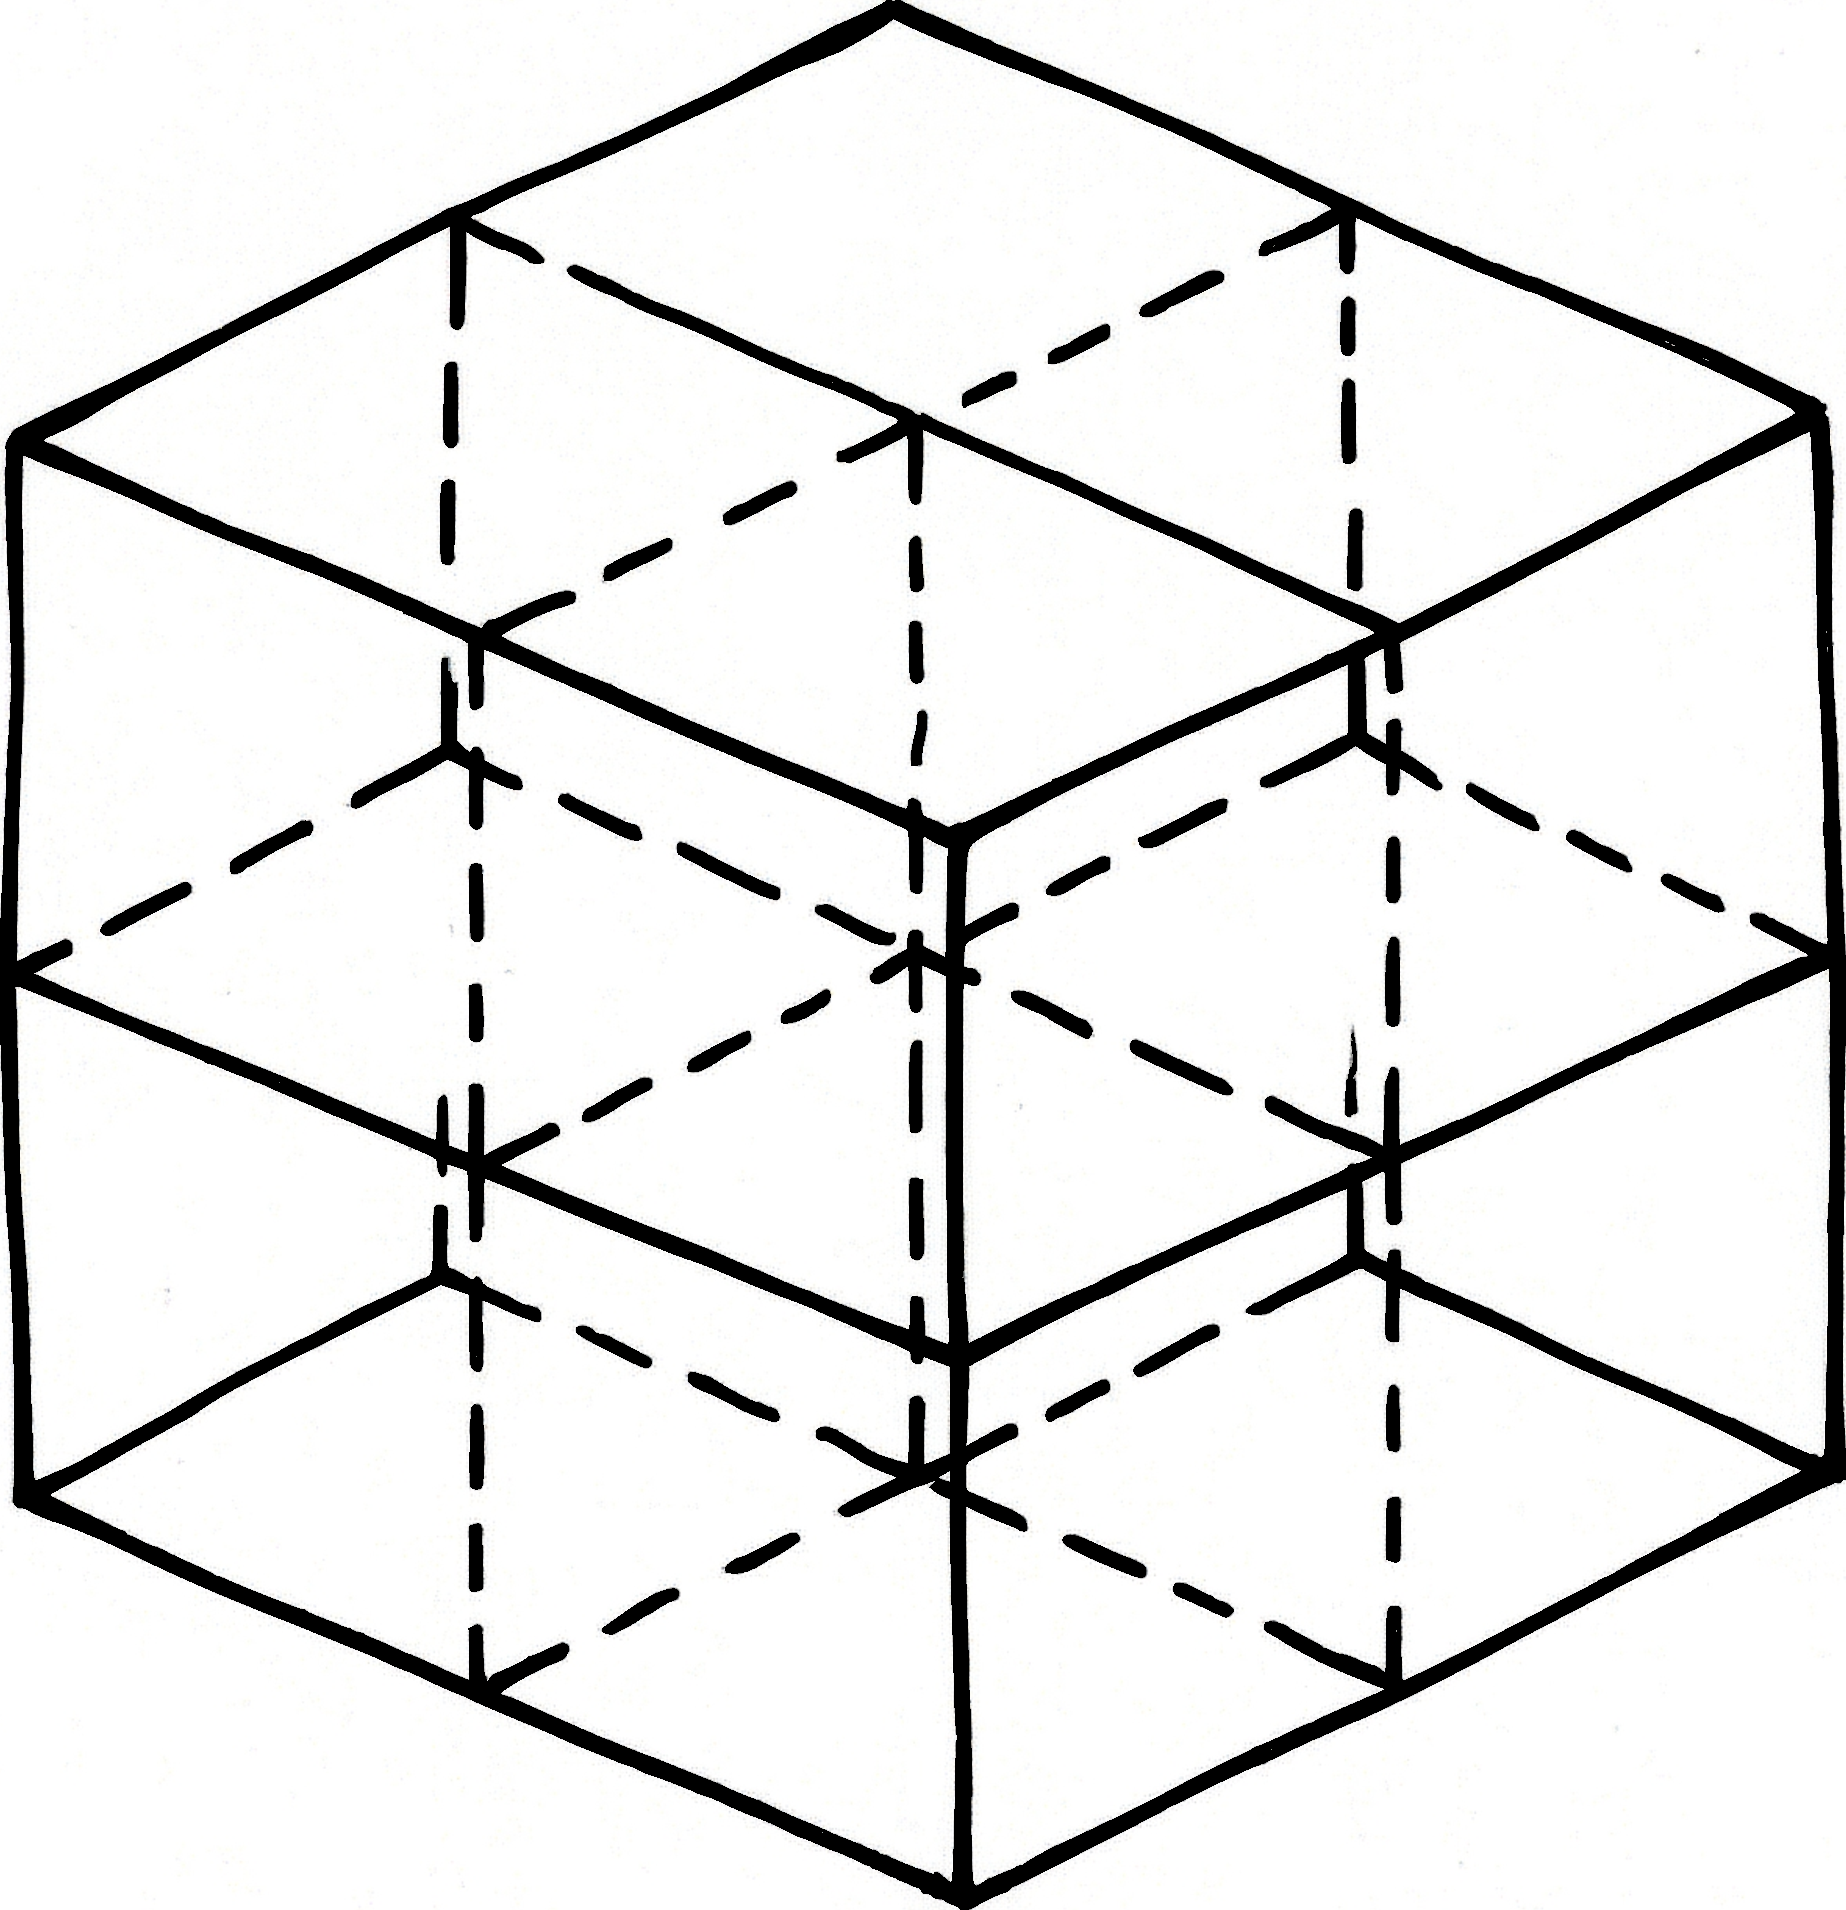
\includegraphics[width=0.3\textwidth]{./assets/cube_perfect_partitioning.pdf}
\end{figure}

However, supposing $n_{processes} = 27$ for the same configuration, the perfect
partitioning requires $3$ (since $3^3 = 27$) workers in each axis, which would
lead to:
\begin{gather*}
  size_x = \frac{20}{3} \approx 6.67 \\
  size_y = \frac{20}{3} \approx 6.67 \\
  size_z = \frac{20}{3} \approx 6.67
\end{gather*}

which is infeasible for a discrete problem. Thus, in order to solve that:
\begin{gather*}
  size_x = \lfloor \frac{20}{3} \rfloor = 6 \\
  size_y = \lfloor \frac{20}{3} \rfloor = 6 \\
  size_z = \lfloor \frac{20}{3} \rfloor = 6
\end{gather*}
However, that also leads to its own issue: the domain is $20 \times
20 \times 20$ computational units wide,
but only $18 \times 18 \times 18$ ($6$ for each worker in the same
axis) \glspl{sample} are being processed.
The worker responsible for handling the end of the domain is thereby
assigned the remainder \cite{grama2003},
that is, $20 \bmod 3 = 2$ extra units for the last processes of each
dimension, ensuring the entire grid is properly computed.

\section{Ghost Cells}
\label{sec:ghost_cells}
This method consists in allocating additional space for
\textit{ghost cells} around the edges of each computational chunk,
extending the computational grid of a worker with the \gls{halo} of its
neighbours, as shown in figure \ref{fig:halo_exchange}
\cite{ghost_cells}. Although these
extra cells are not modified by the local stencil computation, the
memory tradeoff is justified, given that it mitigates
the latency costs of retrieving the data only when it is immediately
required.

\begin{figure}[H]
  \centering
  \caption{Halo exchange between neighboring processes \cite{ghost_cells}}
  \label{fig:halo_exchange}
  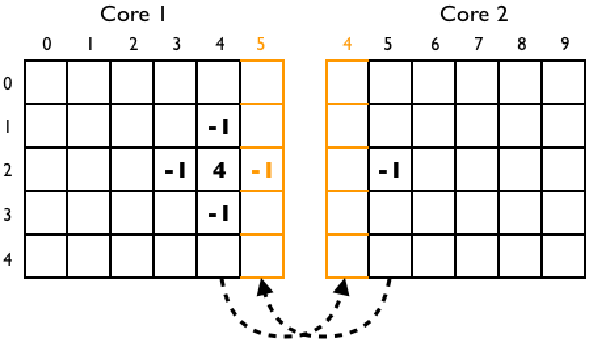
\includegraphics[width=0.6\textwidth]{./assets/ghost_cells_exchange.pdf}
\end{figure}

Such method is often combined with the use of asynchronous
communication, in order to
attain greater performance gains. By using non-blocking message passing,
one can overlap the retrieval of their ghost cells with computation, effectively
reducing potential network bottlenecks, depending on the equilibrium between
compute and network capacity.

\section{Fletcher modeling}
\label{sec:fletcher_modeling}
Reverse Time Migration (RTM), of which Fletcher consists, is defined
as a seismic imaging method to map the subsurface reflectivity using recorded
seismic waveforms \cite{rtm}. In petroleum
exploration, the wave is emitted at the vessel and propagates
outwards in a radial manner, eventually reflecting, in the subsurface, at
velocity boundaries until it is recaptured at sea level.

Such process requires, therefore, that the wave be propagated forward in time
(from $t = 0$ to $t = T$) and backwards (from $t = T$ to $t = 0$)
simultaneously,
so that both models can be cross-correlated with respect to a certain
$t$, making
it feasible to reconstruct the depth and the location of the moment the echoes
crashed.

The hardship, however, arises when dealing with anisotropic media.
Isotropy occurs when
physical properties are shared along all axes, as defined by the
acoustic equation:
\begin{equation}
  \frac{\partial^2 p}{\partial t^2} = v^2 \nabla^2 p
\end{equation}
where $p(x, y, z, t)$ represents the pressure and $v(x, y, z)$ is the
velocity at each point in the grid \cite{fletcher_modeling}.

Nonetheless, when dealing with anisotropy, which is defined by the parameters
$\epsilon(x, y, z)$ and $\delta(x, y, z)$ \cite{anisotropy}, the
symmetry axis is tilted, being characterized by an azimuth ($\phi$)
and dip ($\theta$) angle. When $\phi = \theta = 0$, \acrfull{vti}
occurs, implying that the physical properties are equal along the $x$
axis, but vary throughout the $y$. This happens due to the natural
process of sedimentation, where rocks are formed by the accumulation
of matter over time, creating solid, vertically stacked layers.

Furthermore, due to natural geological events, such as tectonics,
$\phi$ and $\theta$ may not be equal to $0$, leading to a tilted
symmetry axis \cite{fletcher}. In this context of anisotropy, waveforms $P$ and
$S$ are defined: the former shifting in the same direction as
propagation and the latter moving perpendicularly to it
\cite{fletcher}. In this sense, two different velocities are
established: $v_{pz}$ (for $P$) and $v_{sz}$ (for $S$)
\cite{fletcher_modeling}, which are later used by Fletcher through
the establishment of pseudo-acoustic equations:
\begin{gather}
  v_{pn}(x, y, z) = v_{pz}(x, y, z)\sqrt{1 + 2\delta(x, y, z)} \\
  v_{px}(x, y, z) = v_{pz}(x, y, z)\sqrt{1 + 2\epsilon(x, y, z)}
\end{gather}
which act as intermediary variables in order to simplify the
equations for the propagation of pressure $p$ with auxiliary field
$q$ \cite{fletcher_modeling, fletcher}:
\begin{gather}
  \frac{\partial^{2}p}{\partial t^{2}} = v_{px}^{2}H_{2}p + \alpha
  v_{px}^{2}H_{1}q + v_{sx}^{2}H_{1}(p - \alpha q) \\
  \frac{\partial^{2}q}{\partial t^{2}} =
  \frac{v_{pn}^{2}}{\alpha}H_{2}p + v_{px}^{2}H_{1}q -
  v_{sx}^{2}H_{2}(\frac{1}{\alpha}p - q)
\end{gather}
where $\alpha$ is a coupling parameter, typically set to $1$, as suggested
by Fletcher, in order to define the differential operators $H_1$ and
$H_2$ \cite{fletcher}:
\begin{equation}
  \begin{aligned}
    H_{1} = &\sin^{2}\theta \cos^{2}\phi \frac{\partial^{2}}{\partial
    x^{2}} + \sin^{2}\theta \sin^{2}\phi \frac{\partial^{2}}{\partial
    y^{2}} + \cos^{2}\theta \frac{\partial^{2}}{\partial z^{2}} \\
    &+ \sin^{2}\theta \sin 2\phi \frac{\partial^{2}}{\partial x
    \partial y} + \sin 2\theta \sin \phi \frac{\partial^{2}}{\partial
    y \partial z} + \sin 2\theta \cos \phi
    \frac{\partial^{2}}{\partial x \partial z}
  \end{aligned}
\end{equation}

\begin{equation}
  H_{2} = \left( \frac{\partial^{2}}{\partial x^{2}} +
    \frac{\partial^{2}}{\partial y^{2}} + \frac{\partial^{2}}{\partial
  z^{2}} \right) - H_{1}
\end{equation}
which represent, respectively, the anisotropy and the isotropy components
used to solve the pseudo-acoustic equations.

\chapter{Related work}
\label{ch:related_work}
The present work, which employs seismic computation through the lens of
multi-GPU and MPI implementations with ghost cells, has already been
explored by authors in some capacity from varying points of views.
For the purpose of defining this research's value and singularity in such
a landscape, some well-established works ought to be explored, aiming at
providing essential background and inspiration.

\section{Multi-GPU Fletcher}
\citeonline{multi-gpu} explores the distribution of the computation
workload of Fletcher
throughout multiple GPUs, aiming at analyzing its performance through the lens
of scalability and efficiency when compared to its single GPU
baseline counterpart. Similarly to the present work, the domain must
be partitioned between the GPUs (which would be equivalent to workers in MPI),
implying additional synchronization and communication efforts required.

In this sense, the multi-GPU implementation is closely related to the
present one:
the grid is initially partitioned in the $z$ axis, in order to
maximize the use
of the device's L1 and L2 caches. Then, during the actual
computation, ghost cells are used to synchronize the halo regions,
employing device-to-device memory transfers for communication.

Finally, the results reveal a speedup of 2.77 for certain grid sizes,
displaying a linear growth of performance and efficiency as the input size
increases. This, however, is severely degraded for small grids, since GPU
latency, combined with synchronization and communication, easily become the
bottlenecks of the application, becoming computational overheads rather than
required efforts for performance gains. This phenomenon is intrinsically present
in the present MPI implementation at a much greater scale, since
network bandwidth and latency are far more noteworthy bottlenecks
than PCIe transfers, requiring more thorough efforts to mitigate them.

\section{Stencil communication in heterogeneous supercomputers}
\citeonline{stencil_supercomputers} discusses the optimization of
work distribution along a Cartesian grid, emphasizing its importance
in communication-heavy applications, especially when executed on heterogeneous
HPC clusters. The approach consists of a three-step process employing CUDA and
MPI with the goal of distributing work in a node-aware manner whilst leveraging
the most out of the GPUs present in each host.

Akin to this research, the aforementioned approach initiates by partitioning the
domain in order to minimize data exchange. In this context, the immediate goal
is to minimize the surface-to-volume ratio, since halo communications happen on
the faces of the mesh, whilst the computation itself depends directly
on its volume,
leading to an $O(n^2)$ and $O(n^3)$ growth, respectively. Therefore,
it is imperative
to proceed in a manner that directs the greater increase to the part
of the grid that
does not constitute a halo region, thus leading to decomposition in
smaller cubes.
In order to accomplish so, the domain is repeatedly partitioned among
the longest
dimension by the prime factors of the number of nodes sorted in descending order
\cite{stencil_supercomputers}, until the grid is completely
partitioned. Finally,
each unit undergoes the same process for the purpose of distributing
work among a
host's GPUs, as shown in figure \ref{fig:node_decomposition}.

\begin{figure}[H]
  \centering
  \caption{Decomposition of $24$ nodes \cite{stencil_supercomputers}}
  \label{fig:node_decomposition}
  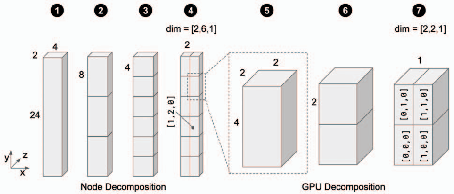
\includegraphics[width=0.75\textwidth]{./assets/supercomputers_domain_decomposition.pdf}
\end{figure}

Subsequently, after the topology has been properly projected on the input mesh,
it is vital to assign the most proper nodes to certain chunks of data, based
on optimization algorithms run on the underlying platform.
In this sense, it is sensible to model the topology as a bijector assignment
between $n$ facilities and $n$ locations, with the goal of placing
the facilities
with the highest flow between them close to one another
\cite{stencil_supercomputers}.
Such optimization problem may be applied to GPUs, aiming at placing
subdomains with
wider halos on GPUs with higher communication bandwidth
\cite{stencil_supercomputers}.
Supposing that $w$ represents the flow matrix between facilities $i$
and $j$, and $d$
represents the distance between locations $i$ and $j$, it is then viable
to model the cost function with $f$ being the bijection between factories and
locations:
\begin{equation}
  w_{i, j}d_{f(i), f(j)} \quad \text{s.t.} \quad i, j \in [0, n)
\end{equation}
which can then be minimized to find the optimal $f$ assignment. Notably,
this is an np-hard problem, implying the need for integer programming
or brute force algorithms. The article in question chooses the latter,
due to the search space for GPUs usually not being high enough to justify
employing more advanced strategies.

Ultimately, once every node and GPU has its share of the domain
assigned to them,
it becomes necessary to decide on the communication strategy to be elected.
This is based on multiple possible scenarios, such as a process being its own
neighbor (no device-to-device transfers needed), multiple processes residing
on a single node (no MPI calls needed, only CUDA IPC instructions) or
many subdomains
in the same MPI process (direct device-to-device communication
through PCIe buses). Such approach leverages the most out of each distinct
circumstance, maximizing the use of the heterogeneity of the HPC cluster.

\section{Accelerating simulation of seismic wave propagation}
\citeonline{okamoto2010} discusses optimization strategies for
seismic applications
based on GPUs from the viewpoint that the numerical complexity of the arithmetic
required is very low, posing little to no issue for the device's hardware. Such
idea thereby leads to the prospect of optimizations on the memory
management side,
implying reduced bandwidth and latency costs. In this sense,
\citeonline{okamoto2010}
leverages the GPU's shared memories and registers by processing 2D blocks one
at a time, leaving the $XY$-plane in the shared memory whilst having
the rest reside
in the registers \cite{okamoto2010}. At the end of an iteration,
these two blocks of
data are swapped, implying no accesses to the notoriously slower global memory.

This approach, however, does not scale well with larger problem
sizes, since the VRAM associated with a single GPU is quickly exhausted.
\citeonline{okamoto2010} discusses, therefore, employing a multi-GPU topology,
making use of MPI for device-to-device data transfers, leveraging halo regions
(referred to as "ghost points" by the authors) and asynchronous
communication for computation overlapping.

Finally, \citeonline{okamoto2010} observes a scaling of $N^{\frac{2}{3}}$
for the problem,
where $N$ is the number of GPUs. Notably, this is due to delays
introduced by communication and computation of halo regions, which also
damages the executions of smaller problem sizes, since latency prevails
in these scenarios. Therefore, \citeonline{okamoto2010} highlights the need
for further optimization on the memory mapping of ghost points, in order
to attain greater results.

\section{Present work}

This research conceives a multi-node MPI implementation of the
Fletcher application \cite{fletcher_modeling} with 3D block
decomposition \cite{stencil_supercomputers} and asynchronous ghost
cell communication \cite{ghost_cells}, addressing the memory
scalability concerns identified by \cite{multi-gpu, okamoto2010} and
enabling the distribution of the computation across several machines
whilst overlapping halo exchanges with the stencil kernel.

In addition, a calibrated SimGrid simulation framework \cite{simgrid}
is provided, allowing the exploration of platform configurations and
network bandwidths beyond those physically available, making up for
the sub-linear scaling limitations observed by \cite{okamoto2010}
through capacity planning on larger interconnection networks.

\chapter{Parallel application design with ghost cells}
\label{ch:application_design}

This chapter details the design and implementation of the distributed
Fletcher application. It begins with the static partitioning strategy
using MPI Cartesian topologies, followed by the initialization and
finalization procedures of the coordinator-worker model. Next, the
communication scheme based on asynchronous ghost cell exchanges is
described, along with the main computation loop that overlaps halo
transfers with stencil processing. The chapter then covers the GPU
acceleration via CUDA, the numerical validation against the reference
implementation, and concludes with the SimGrid-based simulation
methodology.

\section{Static partitioning with MPI}
The application was built from using OpenMPI as the
messaging interface, aiming at a reliable and well-established
distributed computation framework.

The study of adapting the Fletcher application for execution in cluster
environments with MPI-based libraries involves determining how the
three-dimensional problem domain will be partitioned. Figure
\ref{fig:partitioning_methods} illustrates three possible strategies
identified (from left to right) as Slices, Columns and Blocks.

\begin{figure}[H]
  \centering
  \caption{Three partitioning strategies for a 3D domain: by slices
  (left), by columns (center) and by blocks (right). (source: the author)}
  \label{fig:partitioning_methods}
  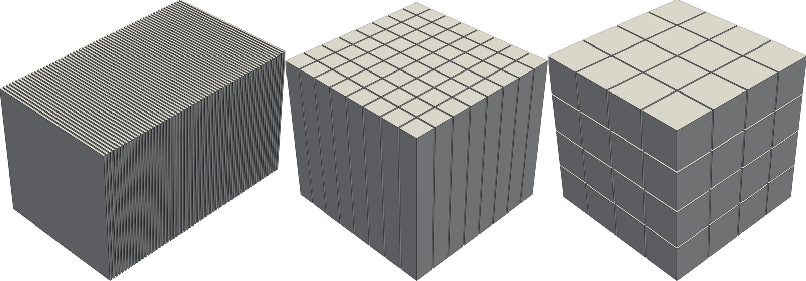
\includegraphics[width=0.9\textwidth]{./assets/partitioning_methods.pdf}
\end{figure}

The implications of each partitioning strategy on communication cost
must be considered, since communication directly affects the scalability
and efficiency of parallel processing. In the Fletcher computation
kernels, partitions must constantly exchange data about what happens at
their boundaries. As shown in Figure
\ref{fig:comms_vs_partitioning}, if the partitioning strategy is
inefficient (such as Slices), the contact surface between processors
grows linearly ($2(P - 1)L^2$, where $P$ is the number of processors
and $L$ is the cube width), creating a bottleneck where the time spent
moving data across the network surpasses the time spent on actual
computation. By opting for more compact strategies, such as Blocks
($6(\sqrt[3]{P} - 1)L^2$), this boundary area is minimized, ensuring
that the system spends most of its time computing and allowing
performance to continue increasing as more processors or accelerators
are added.

\begin{figure}[H]
  \centering
  \caption{Comparing the communication cost (Y axis) generated by the
    three partitioning strategies from Figure
    \ref{fig:partitioning_methods} (color) as a function of the number
  of processors (X axis). (source: the author)}
  \label{fig:comms_vs_partitioning}
  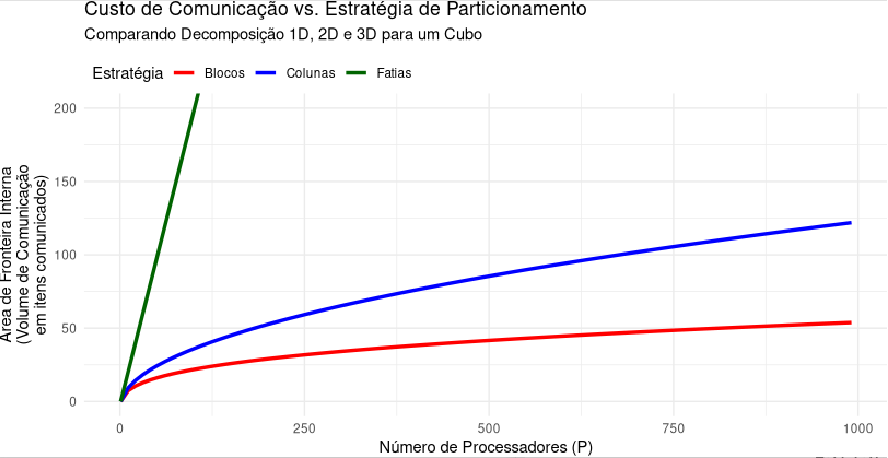
\includegraphics[width=0.9\textwidth]{./assets/chart_comms_vs_partitioning.pdf}
\end{figure}

Thus, among the various possible strategies, a 3D Block partitioning
is chosen given that it always generates a smaller communication
boundary. The first and arguably most important step of the program is
thereby to assign partitions of the domain to the available workers.
This is accomplished through the use of MPI's
\lstinline{MPI_Dims_create()} function, a convenience function that
automatically calculates how to divide the total number of processes
across X, Y and Z so that the domain is as balanced and cubic as
possible \cite{grama2003}. It seeks to minimize contact surfaces (the
boundaries) without the need for manual partitioning calculations,
ensuring that the workload is distributed in the most compact form
possible. It is noteworthy, however, that this does not handle the
segmentation of the problem domain itself, but rather only distributes
the available workers across the Cartesian grid.

When the number of processes is prime (e.g., 7, 13, 17),
\lstinline{MPI_Dims_create} cannot factor them into a balanced cube or
block. In such cases, it is forced to generate a 1D partition
(Slices), resulting in something like $\{17, 1, 1\}$ for 17 processes.
This ``worst case'' for efficiency, which maximizes the boundary area
and communication cost as shown in Figure
\ref{fig:comms_vs_partitioning}, should be avoided by always choosing
a number of processes that is a power of 2 or highly composite (such
as multiples of 2, 3 and 5), ensuring that the algorithm can create
compact and balanced subdomains.

The aforementioned partitioning, combined with \lstinline{MPI_Cart_create()},
creates a global communicator through which all processes will pass messages
for the rest of the program's lifespan. Furthermore, the concept of neighborhood
is provided: each process possesses, henceforth, its own coordinates, defined by
\lstinline{MPI_Cart_coords}. By combining this with \lstinline{MPI_Cart_rank},
which provides the rank of the process assigned to a certain set of coordinates,
a worker has the ability to receive messages from and send messages
to its surrounding
neighbors.

Furthermore, the mapping from the neighboring index $i \in [0, 27)$ to a
displacement $d \in \{-1, 0, 1\}$ from the source is given by:
\begin{equation}
  \begin{cases}
    d_x = i \bmod{3} \\
    d_y = \lfloor (i \bmod{9}) / 3 \rfloor \\
    d_z = \lfloor i / 9 \rfloor
  \end{cases}
\end{equation}

Since $d_x, d_y, d_z \in \{0, 1, 2\}$, an offset is added so
the set centers around $0$, representing the current process.
With $d_x, d_y, d_z \in \{-1, 0, 1\}$, the neighbor's coordinate is
thereby calculated as:
\begin{equation}
  \vec{C}_{neigh} = \vec{C}_{self} + (d_x - 1, d_y - 1, d_z - 1)
\end{equation}

\section{Initialization and finalization}
The application operates with a coordinator-worker model based on MPI.
Before the domain partitioning takes place, all processes---including
the \gls{coordinator}---execute a common preparation: each one discovers
the total number of participants, distributes that total automatically
into a three-dimensional process grid and initializes the internal
structures that describe its position in that grid, its immediate
neighbors and the physical parameters of the simulation. The global
domain is expanded to accommodate absorption zones at the borders and
additional cells required by the eighth-order finite difference scheme.

\subsection{Coordinator: partitioning and dispatch}
The coordinator is responsible for partitioning the cube,
effectively deciding which worker computes which part of the grid.
The division is performed by subtracting the border cells from the
total domain and distributing the remainder equally among the processes
of each dimension. The integer remainders of this division are absorbed
by the processes at the final position of each axis.
The coordinator also locates the seismic source, positioning it at the
geometric center of the global domain (as per the reference
implementation), and verifies whether it falls within its own
sub-volume; for the remaining processes, the verification is performed
during the dispatch of partition information.

With all partitions calculated, the coordinator systematically
traverses all processes in the three-dimensional grid and sends each
one, individually, a compact metadata packet describing its sub-cube:
local and global dimensions, starting coordinates in the global
domain, number of time iterations, seismic source position (if it
belongs to that sub-cube) and absorption zone size. The dispatch
consists of a single data block per recipient; no wavefield vectors are
transmitted, since each process initializes its own sub-volume locally
after receiving these metadata.

After distributing the information, the coordinator allocates its own
wavefield vectors and initializes the velocity model and the
anisotropy coefficients for its sub-volume, in the same manner as the
workers.

\subsection{Workers: awaiting data}
The workers begin their execution by synchronously
awaiting the arrival of the partition metadata sent by the
coordinator. Upon receiving this packet, each worker knows exactly the
dimensions of its block, its position in the global domain and the
number of time steps to execute.

With this information in hand, the worker allocates the four wavefield
vectors necessary for the propagation---two for the $P$ field and two
for the auxiliary $Q$ field, representing the past and current instants
in each case. All vectors are initialized with zeros. Next, the worker
fills its sub-volume's anisotropy model with default velocity values
and applies a random variation in the border and absorption zones,
using the global starting coordinates received to ensure consistency
with what would be produced by a single centralized model (such as
the reference program). Finally, the spatially variant anisotropy
coefficients (described in Section~\ref{sec:fletcher_modeling}),
derived from the tilt and azimuth angles of the local velocity model,
are precomputed and will be used repeatedly during the propagation.

This independent computation of anisotropy variables by each process
leverages the advantages of splitting memory in a distributed setup,
preventing \acrshort{oom} interruptions on the coordinator.

\subsection{Finalization}
By the end of the execution, once all workers are finished with their
chunks of the domain, they send their share of the data to the
coordinator, which takes turns in receiving and flushing the received
parts, effectively avoiding the need to concentrate the entire cube in
RAM.

\section{Communication}
The application utilized both synchronous and asynchronous
communication, using the most proper approach depending on the scenario
requiring it.

Synchronous communication is scarcely used in the program, being employed
solely at synchronization points, behaving akin to barrier mechanisms.
The only events that represent that scenario are the initialization
and the finalization, since these are defined by the distribution and
the reassembling of data, respectively. In such context, synchronous
communication
offers greater integrity, since it prevents data corruption caused by
the premature
use of receiving buffers.

Asynchronous communication, on the other hand, is the core of the
program, essential to accomplishing the goal of overlapping
communication with computation, greatly backed
by the use of ghost cells (Section~\ref{sec:ghost_cells}).
All workers operate on an extended version of their domain, which
includes their own partition with the addition of their neighbors'
borders. This version is present to the processes before the processing
iterations begin. Figure~\ref{fig:ghost_cells_cubes} (left) illustrates
a scenario of $4 \times 4 \times 4 = 64$ processes where each block
possesses ghost cells around its perimeter. In practice, the right image
of Figure~\ref{fig:ghost_cells_cubes} illustrates what occurs, where
there is no data replication on the outer part of the problem domain
(entire cube), and the ghost cells of the inner part are communicated in
a specific order asynchronously.

\begin{figure}[H]
  \centering
  \caption{On the left image, in each block, the gray interior
    represents the part of the domain that the process actually
    computes, while the orange shell (Ghost Cells) represents the
    additional memory needed to store data coming from neighbors that
    enable the computation of the interior. On the right image,
    different colors (Orange for X, Green for Y, Blue for Z) illustrate
    that, in MPI, the communications typically occur in separate
  stages. (source: the author)}
  \label{fig:ghost_cells_cubes}
  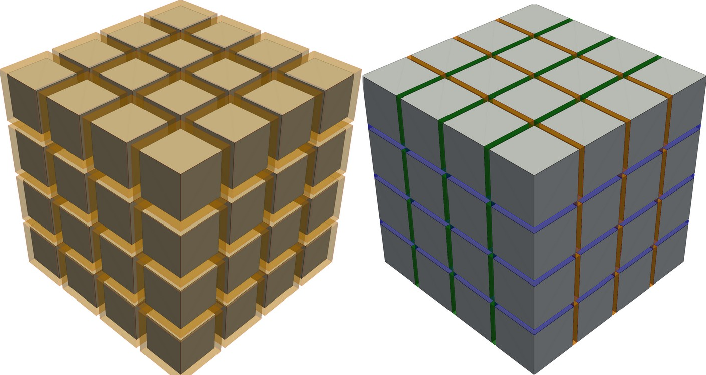
\includegraphics[width=0.9\textwidth]{./assets/ghost_cells_cubes.pdf}
\end{figure}

\subsection{Main computation loop}
Upon completion of the initialization phase, coordinator and workers
converge to the same execution path: all process their own block
through the same wave propagation method. There is no functional
distinction between the coordinator and the remaining processes during
the time loop. The coordinator simply operates on the partition
corresponding to its position in the 3D Cartesian grid, just like any
other process.

Each process measures the execution time of the propagation loop to
report performance in samples/second at the end. When all iterations
complete, each process sends its final results to the coordinator,
which collects and writes the binary output file.

If we suppose $t$ to be the current timestamp, at $t = T$, a process:

\begin{enumerate}
  \item Inserts the source of the pseudo-acoustic wave in its own domain.
  \item Begins an asynchronous receive of the borders of $t = T + 1$.
  \item Computes its own borders (the ones its neighbors need).
  \item Asynchronously sends its borders to the neighbors.
  \item Computes its interior.
  \item Waits for the received ghost cells and inserts them.
  \item Swaps wavefield vectors.
  \item Waits for the asynchronous sends to finish.
  \item Proceeds to $T + 1$.
\end{enumerate}

It is noteworthy that all these operations are local activities
involving a block and its immediate neighbors, which enables
parallelism of both computation and communication. Each step is
described in more detail below.

\textbf{Seismic source injection.}
At the beginning of each time step, the process that contains the
seismic source position in its sub-volume injects a Ricker wavelet---the
second derivative of a Gaussian. This pulse, whose value depends on
the current time instant and a predefined cutoff frequency, is added
simultaneously to both wavefield arrays, $P$ and $Q$, at the
corresponding position in the local vector.

\textbf{Asynchronous reception of ghost cells.}
Immediately after adding the source, the process launches non-blocking
receive operations for the halo data (ghost cells) that will come from
each of the up to twenty-six possible neighbors in the three-dimensional
grid. Each expected ghost cell has a size determined by the stencil
thickness in the dimensions where there is adjacency and by the
computable extent in the remaining ones. The receives are initiated
without waiting for their completion, allowing local processing to
progress while data is still in transit.

\textbf{Boundary computation.}
With the asynchronous receives underway, the process computes the
boundary regions of its block---the internal strips closest to each
face, whose values will be sent as ghost cells to the neighbors. The
domain is divided into low and high boundaries on each of the three
axes, with overlaps avoided by careful staggering of regions. When the
block is too small for this separation, the entire domain is computed
at once (effectively disabling ghost cell overlap). The effective
propagation uses the eighth-order finite difference scheme to update
the wavefields, as per the original reference program.

\textbf{Asynchronous send of computed boundaries.}
As soon as the boundary regions are updated, the process extracts each
relevant boundary strip into a contiguous buffer and launches
non-blocking sends to each corresponding neighbor. The buffers are
accumulated for later release, when the sends are confirmed. This
dispatch covers both pairs of fields---past $P$ and past $Q$---since
these are the values that neighbors need to compute the next iteration.

\textbf{Interior computation.}
With the sends already underway, the process computes the central
region of the block, which will not be communicated in this iteration.
This region is larger and concentrates the bulk of the computational
work. By processing it while the halos travel across the network, the
application overlaps communication and computation, reducing idleness.

\textbf{Waiting for received ghost cells.}
After completing the interior, the process waits for the arrival of
all ghost cells sent by the neighbors, unifying into a single
collective wait the handles of the receives for both fields. Only when
all data is available does the iteration advance.

\textbf{Ghost cell insertion into local vectors.}
With the ghost cells received, their data is written into the ghost
cell positions of the block. Values from a neighbor on the left fill
the first cells of the corresponding axis; those from the right fill
the last; and those from neighbors with no displacement on that axis
fill the intermediate strip. This operation restores consistency at the
sub-volume borders so that the finite difference stencil can operate
correctly in the next iteration.

\textbf{Vector swap.}
With the wavefield updated, the roles of the two pairs of vectors are
inverted: the vector that contained the past values now points to the
newly computed values, becoming the new present; the one that was the
present becomes the recipient for the next update. This swap is
performed by exchanging pointers only, without any data copy, keeping
the cost of the operation constant and minimal.

\textbf{Final wait for sends.}
Lastly, the process waits for the completion of all asynchronous sends
initiated during the iteration. Only after this confirmation are the
send buffers released. This concludes the current iteration, and the
loop advances to the next time step.

The above process can be translated into the following pseudocode:
\begin{lstlisting}[style=CStyle, caption = {Main worker loop using Ghost Cells}]
double dc_worker_process(problem_data data, unsigned int iterations) {
  for (unsigned int i = 0; i < iterations; i++) {
    add_source(data);

    problem_data future_halos = async_receive_halos();

    compute_boundaries(data);

    async_send_halo_to_neighbours(data);

    compute_interior(data);

    merge_halos(data, future_halos);

    wait_async_requests();
  }
}
\end{lstlisting}

This ensures that while the operating system handles the asynchronous
network calls, the program continues to process its domain, effectively
overlapping communication with computation.

\section{GPU acceleration via CUDA}
\label{sec:gpu_cuda}
The local clusters at the Institute of Informatics predominantly
feature Nvidia accelerators; for this reason, the porting of the
propagation kernels to the MPI implementation was carried out via the
CUDA API. Although this specificity exists, it is understood that
substitution by another API such as HIP would be very similar given the
same host-device programming model with accelerators.

\subsection{Compilation differences}
The application supports two major computation modes: one based on CPU
with thread parallelism (OpenMP) and another that delegates the
wavefield computation to the GPU via CUDA. In the CPU mode, all code
is compiled by a conventional MPI compiler, and the parallelism within
each process is managed by pragma directives that distribute loops
among the available cores.

In the GPU mode, the files that implement the field propagation and
device memory management are compiled by the NVIDIA compiler, with
code generation for the specified target architecture. The resulting
objects are linked to the rest of the program by the same MPI compiler
used in the CPU mode, with the CUDA runtime libraries included in the
linking step. The interface between C code and CUDA code is protected
by linkage guards that prevent compatibility issues between the two
compilers.

Throughout the simulation in GPU mode, the wavefield vectors reside in
device memory. Only the MPI communication buffers travel between host
and device, during the ghost cell extraction and insertion operations,
carried out through three-dimensional strided copies that avoid
unnecessary data reorganizations.

When multiple MPI processes reside on the same node, the GPU assigned
to each process is selected automatically based on the hostname: the
processes on the same node are distributed cyclically among the
available GPUs, ensuring that the load is balanced without manual
configuration.

\subsection{Kernel comparison with reference implementation}
The propagation kernel of this project was redesigned relative to the
reference implementation to meet the requirements of distributed
execution. The most important difference is that this project's kernel
operates on parameterizable sub-regions of the local domain: by
receiving start and end coordinates, it can be invoked separately on
the boundaries and on the interior, enabling the overlap of MPI
communication with GPU computation---the same overlap mechanism present
in the CPU backend.

In the reference implementation, the kernel always operates on the
complete domain minus a fixed border strip, without the possibility of
selecting sub-regions. It was designed for single-process execution,
without MPI coordination, so there is no need to distinguish interior
from border for communication purposes.

Another relevant difference concerns the anisotropy coefficients. In
this project, these coefficients are treated as compile-time constants,
calculated from simplified isotropic assumptions; the kernel receives
only the essential velocity vectors and derives the remaining
parameters internally. In the reference implementation, all ten
coefficient vectors are passed explicitly to the kernel as pointers to
device memory, which increases flexibility for models with spatially
variable anisotropy but also raises the number of parameters and the
pressure on GPU registers.

The thread block size also differs: this project uses square blocks of
sixteen by sixteen threads, with an explicit guard to handle domains of
arbitrary size; the reference implementation uses blocks of thirty-two
by sixteen and requires domain dimensions to be exact multiples of
those values. The device variables in the reference are global and
static, shared across all invocations; in this project, each MPI
process possesses its own device data structure, encapsulating
allocation and pointers independently and safely for multi-process
execution.

\section{Numerical validation}
In order to guarantee that the present MPI implementation properly
addressed the base
program, it was imperative that the numerical results produced
properly matched the reference. Therefore, several runs with different
amount of workers, problem sizes and iterations were executed both in the
MPI and in the base version. Then, the SHA-256 checksum of both were
compared against each other, in order to attain a reliable and reproducible
validation process.

In this context, Table~\ref{tab:openmp_validation} summarizes the
OpenMP validation scenarios. For each combination, the SHA-256
checksum of the MPI output was compared against the single-node
reference. All checksums matched exactly, indicating flawless
numerical precision for the OpenMP backend.

\begin{table}[H]
  \centering
  \caption{OpenMP numerical validation scenarios executed on an AMD
    Ryzen~5 7600 at 5.17~GHz, all with 10 iterations. Every scenario
  produced an identical SHA-256 checksum to the single-node reference.}
  \label{tab:openmp_validation}
  \begin{tabular}{ll}
    \hline
    Parameter & Values \\
    \hline
    Workers       & 1, 2, 3, 4, 5, 6 \\
    Problem sizes & $32^3$, $64^3$, $128^3$, $256^3$, $512^3$ \\
    Iterations    & 10 \\
    \hline
    Total scenarios & $6 \times 5 = 30$ \\
    Matching checksums & 30 / 30 \\
    \hline
  \end{tabular}
\end{table}

The CUDA version, however, required a delta-based approach, since tiny numerical
differences are expected due to hardware differences in floating
point arithmetic, such as \acrfull{fma},
between the CPU and the GPU, as documented in the IEEE 754 compliance
standards. Therefore, the MPI CUDA version was compared to
the ground truth within a small tolerance ($10^{-15}$), having
succeeded in such comparison. It is noteworthy, however, that such
tiny differences eventually accumulate through iterations:
\begin{equation}
  E_{total} \approx \sum_{t = 1}^{n}{\delta_t}
\end{equation}
where $\delta_t$ is the error introduced by each time step,
which leads to the accumulated error being a linear function in
respect to time.

\section{Simulation}
The present project aimed at providing a simulation tool in addition
to the implementation
of the MPI application, with the goal of finding optimal environments and
configurations for the program to run with.
The simulations are handled by SimGrid \cite{simgrid} by modeling the target
HPC cluster's network topology through the
\href{https://simgrid.org/doc/latest/app_s4u.html}{S4U}
interface and providing the nominal bandwidth and latency values to the
program, which proceeds henceforth to execute the application code.

In this scenario, pure sampling methods were tested for the purpose of
accelerating the simulation. One such approach, for instance, was to
replace every computation call with a sampling function that merely executed
a certain amount of \acrshortpl{flop}, which value was determined based on
the actual kernel's mathematical operations. This, however, proved to be
a severe oversimplification of the program, reducing it to a pure mathematical
function based on linear and non-linear regressions, which thoroughly
disregarded the complex nature of the application, such as PCIe transfers,
cache hits/misses, memory copies, etc.

For this reason, it was decided to leverage SimGrid's potential to fully emulate
the source code while reducing total simulation time by sampling the
main computation
kernel iteratively until it stabilizes. Appendix
\ref{ap:sampled_comp} demonstrates
how this is performed.

\chapter{Results}
\label{ch:results}

The results obtained by the present research illustrate the use
of the distributed MPI version of Fletcher in real HPC clusters
as well as the application's simulated version, aiming at making
up for the lack of computational resources for further experimenting.

\section{HPC cluster executions}

The experiments cover both CPU and GPU hardwares, highlighting their
implications
in the final result and respective performance analysis.

\subsection{CPU}

The experiments were conducted on the \textit{cei} cluster of the
PCAD. The cluster consists of six computational nodes, connected by
a 10~Gbit network, each equipped with two Intel Xeon E5-2699 at
2.0~GHz, offering 48 threads with 24
cores and a 256~GB DDR4 with a 1.9~TB SSD. The experiments utilize
OpenMP to leverage each node's parallelism capabilities, as well
as Nix for reproducibility. Tracing is handled by akypuera
\cite{akypuera}, which tracks every MPI action performed by
the processes, to be later converted to a single CSV file
describing all MPI operations executed by each rank, using the
PajeNG tool \cite{pajeng}. This file is then subjected to scripts
developed in the R language with the tidyverse/ggplot2 meta-package
for data analysis and computation of masking ratios and performance.

Figure~\ref{fig:real_cpu_gantt_256}
illustrates a space-time chart of a $256 \times 256 \times 256$
problem size execution, reflecting the behavior of each of the ranks
(Y axis) over time (X
axis), with the colors of the rectangles representing which operations
were performed and their durations. Only the first three seconds are shown, in
order to illustrate the overall behavior within the iterations. Although
the chart contains three distinct MPI operations---\texttt{Irecv},
\texttt{Isend}
and \texttt{Waitall}---one can observe that the latter is the most
present in time,
since the other two are practically instantaneous operations. The most relevant
observation to be made here is the predominance of computation over
communication time, which is more clearly observable in
figure~\ref{fig:real_cpu_load_256}:
the aggregate load sits at $\approx 75\%$ compute per quantile, pointing that
a $256^3$ problem size requires more time from an Intel Xeon E5-2699 than from
a 10~Gbit network.

\begin{figure}[ht]
  \centering
  \caption{Gantt and load charts of a $256^3$ problem size execution}
  \begin{subfigure}{\textwidth}
    \centering
    \caption{Gantt chart of a $256^3$ execution}
    \label{fig:real_cpu_gantt_256}
    
\includegraphics[width=\textwidth]{./assets/real_cpu/gantt_256.pdf}
  \end{subfigure}
  \begin{subfigure}{\textwidth}
    \centering
    \caption{Space-time load chart of a $256^3$ execution, split by
    quantiles with the respective load of each operation}
    \label{fig:real_cpu_load_256}
    
\includegraphics[width=\textwidth]{./assets/real_cpu/load_256.pdf}
  \end{subfigure}
\end{figure}

Finally, by observing figure~\ref{fig:real_cpu_gantt_512}, representing
the first five seconds of a $512^3$ execution,
one can notice much longer compute events than MPI events.
In addition, figure~\ref{fig:real_cpu_load_512} reveals an $\approx
87\%$ load from compute alone,
indicating that as problem sizes grow, computation costs increase at a
larger rate than communication ones. In fact, the reasoning is
immediate: block faces grow more slowly ($6(\sqrt[3]{P} - 1)L^2$)
compared to the volume of the cube ($L^3$). Thus, while the
processing capacity grows cubically, the communication requirement (boundary)
grows only quadratically. This allows exploring different
boundary/volume ratios, as presented in
Table~\ref{tab:frontier_volume} for a fixed number of processors
$P = 64$.

\begin{table}[H]
  \centering
  \caption{Boundary/Volume ratio for different block widths $L$ with
  $P = 64$ processors.}
  \label{tab:frontier_volume}
  \begin{tabular}{cccc}
    \hline
    $L$ (Width) & Volume ($L^3$) & Boundary ($18L^2$) & Boundary/Volume Ratio \\
    \hline
    10   & 1\,000           & 1\,800       & 1.80  \\
    100  & 1\,000\,000      & 180\,000     & 0.18  \\
    1000 & 1\,000\,000\,000 & 18\,000\,000 & 0.018 \\
    \hline
  \end{tabular}
\end{table}

Note that by increasing the problem tenfold, the volume (useful work)
increases 1\,000 times, while the boundary (communication cost) increases
only 100 times. This demonstrates that the larger the local problem
(larger $L$) on each processor, the ``cheaper'' communication becomes in
relative terms. The system therefore gains computational efficiency
because the communication/computation ratio tends to zero as the
problem grows.

\begin{figure}[ht]
  \centering
  \caption{Gantt and load charts of a $512^3$ problem size execution}
  \begin{subfigure}{\textwidth}
    \centering
    \caption{Gantt chart of a $512^3$ execution}
    \label{fig:real_cpu_gantt_512}
    
\includegraphics[width=\textwidth]{./assets/real_cpu/gantt_512.pdf}
  \end{subfigure}
  \begin{subfigure}{\textwidth}
    \centering
    \caption{Space-time load chart of a $512^3$ execution, split by
    quantiles with the respective load of each operation}
    \label{fig:real_cpu_load_512}
    
\includegraphics[width=\textwidth]{./assets/real_cpu/load_512.pdf}
  \end{subfigure}
\end{figure}

\subsection{GPU}

The experiments were conducted on the \textit{poti} cluster of the
PCAD. The cluster consists of five computational nodes, each
equipped with an Intel Core i7-14700KF processor at 3.4~GHz, offering
a hybrid architecture of 20 cores and 28 threads. Each machine is
equipped with 96~GB of DDR5 RAM, an NVIDIA GeForce RTX~4070 GPU with
12~GB for hardware acceleration, and a mixed storage system combining
the speed of a 119~GB NVMe with the capacity of a 1.7~TB SSD. The
nodes are interconnected by a Gigabit network. The experiments
described below use all five nodes and employ only the five RTX~4070
accelerators. The same software toolchain described in the CPU
experiments is used for tracing and analysis.

In the figures that follow, each Gantt chart shows only a subset of
the total execution time, chosen for visibility of the individual
iterations; the load charts, on the other hand, always cover the full
execution duration and therefore provide the most meaningful
quantitative perspective.

Figure~\ref{fig:real_gpu_128} presents the Gantt and load charts
for a $128^3$ problem size. The Gantt chart shows the first second
of execution, where \texttt{Waitall} dominates, with computation appearing
as thin slivers between long waiting periods. The load chart confirms
this across the full $\approx 17$~second run: the aggregate compute
load sits at $\approx 20$--$25\%$, indicating that the RTX~4070
finishes its local computation far faster than the Gigabit network can
deliver the ghost cells, leaving each rank idle for the majority of
each iteration.

\begin{figure}[H]
  \centering
  \caption{Gantt and load charts of a $128^3$ GPU execution}
  \begin{subfigure}{\textwidth}
    \centering
    \caption{Gantt chart of a $128^3$ execution (first second)}
    \label{fig:real_gpu_gantt_128}
    
\includegraphics[width=\textwidth]{./assets/real_gpu/gantt_128.pdf}
  \end{subfigure}
  \begin{subfigure}{\textwidth}
    \centering
    \caption{Space-time load chart of a $128^3$ execution, split by
    quantiles with the respective load of each operation}
    \label{fig:real_gpu_load_128}
    
\includegraphics[width=\textwidth]{./assets/real_gpu/load_128.pdf}
  \end{subfigure}
  \label{fig:real_gpu_128}
\end{figure}

Figure~\ref{fig:real_gpu_256} shows the results for a $256^3$
execution. The Gantt chart shows that the compute
segments become more visible compared to $128^3$; however, the load
chart still shows a similar $\approx
20\%$ compute fraction, confirming that the network remains the
bottleneck in these circumstances.

\begin{figure}[H]
  \centering
  \caption{Gantt and load charts of a $256^3$ GPU execution}
  \begin{subfigure}{\textwidth}
    \centering
    \caption{Gantt chart of a $256^3$ execution (first second)}
    \label{fig:real_gpu_gantt_256}
    
\includegraphics[width=\textwidth]{./assets/real_gpu/gantt_256.pdf}
  \end{subfigure}
  \begin{subfigure}{\textwidth}
    \centering
    \caption{Space-time load chart of a $256^3$ execution, split by
    quantiles with the respective load of each operation}
    \label{fig:real_gpu_load_256}
    
\includegraphics[width=\textwidth]{./assets/real_gpu/load_256.pdf}
  \end{subfigure}
  \label{fig:real_gpu_256}
\end{figure}

Finally, figure~\ref{fig:real_gpu_512} presents the $512^3$ case.
The Gantt chart shows wider compute blocks than the
previous sizes, yet \texttt{Waitall} still prevails. Although
Table~\ref{tab:frontier_volume} predicts a decreasing boundary/volume
ratio with larger blocks, the load chart reveals that the compute
fraction remains at $\approx 20\%$,
virtually unchanged from $128^3$ and $256^3$. This indicates that,
despite the volume growing cubically, the RTX~4070 processes even the
larger domain so quickly that the Gigabit network remains the
overwhelming bottleneck. Increasing the problem size alone is
therefore insufficient to achieve masking on this platform.

\begin{figure}[H]
  \centering
  \caption{Gantt and load charts of a $512^3$ GPU execution}
  \begin{subfigure}{\textwidth}
    \centering
    \caption{Gantt chart of a $512^3$ execution (first 3 seconds)}
    \label{fig:real_gpu_gantt_512}
    
\includegraphics[width=\textwidth]{./assets/real_gpu/gantt_512.pdf}
  \end{subfigure}
  \begin{subfigure}{\textwidth}
    \centering
    \caption{Space-time load chart of a $512^3$ execution, split by
    quantiles with the respective load of each operation}
    \label{fig:real_gpu_load_512}
    
\includegraphics[width=\textwidth]{./assets/real_gpu/load_512.pdf}
  \end{subfigure}
  \label{fig:real_gpu_512}
\end{figure}

Further increasing the block size is impractical: the RTX~4070's
12~GB VRAM easily becomes a resource bottleneck, and
experiments still show communication-dominated behavior
on the Gigabit network. The path forward is therefore not to enlarge
the problem, but to improve the interconnection network---a change
that is infeasible on the physical \textit{poti} cluster but readily
explorable through simulation.

\section{Simulation}
\label{sec:simulation_results}
To demonstrate the masking capability of the implemented MPI
program under faster networks, simulations using SimGrid SMPI were
conducted \cite{simgrid}. SimGrid allows controlling the platform
configuration and executing the same application code on a customized
virtual platform: the computation code is effectively executed
(emulation) while the MPI communication directives are simulated.
A single \textit{poti} node was used to run the SMPI simulations so
that the computation times match those obtained on the real platform.

Before running the simulations, the \textit{poti} platform was
calibrated following the methodology described by
\cite{simgrid_calibration}, which details techniques for extracting
and modeling the characteristics of the MPI runtime backend and the
network, such as protocol thresholds, latency and bandwidth,
into accurate SimGrid
platform descriptions. This calibration step ensures that the
simulated computation and communication timings faithfully
reproduce those observed on the real cluster within an error margin
of at most $15\%$ for messages measuring up to $1073741824$ bytes,
the largest size used in the experiments to follow.

Two simulated network configurations were evaluated: 10~Gbps and
100~Gbps, representing a tenfold and hundredfold improvement over the
real Gigabit interconnect, respectively.

Figure~\ref{fig:sim_gpu_10g_256} presents the results for a $256^3$
execution on the 10~Gbps simulated network. The Gantt chart already
shows a reversal compared to the real Gigabit
results (figure~\ref{fig:real_gpu_256}): computation now dominates
each iteration. The load chart confirms
this, with the aggregate compute load rising to $\approx 65$--$70\%$.

\begin{figure}[H]
  \centering
  \caption{Gantt and load charts of a simulated $256^3$ GPU execution
  with a 10~Gbps network}
  \begin{subfigure}{\textwidth}
    \centering
    \caption{Gantt chart of a $256^3$ execution (10~Gbps, first second)}
    \label{fig:sim_gpu_10g_gantt_256}
    
\includegraphics[width=\textwidth]{./assets/sim_gpu_10Gbps/gantt_256.pdf}
  \end{subfigure}
  \begin{subfigure}{\textwidth}
    \centering
    \caption{Space-time load chart of a $256^3$ execution (10~Gbps),
    split by quantiles with the respective load of each operation}
    \label{fig:sim_gpu_10g_load_256}
    
\includegraphics[width=\textwidth]{./assets/sim_gpu_10Gbps/load_256.pdf}
  \end{subfigure}
  \label{fig:sim_gpu_10g_256}
\end{figure}

At $512^3$ on the same 10~Gbps network
(figure~\ref{fig:sim_gpu_10g_512}), the Gantt chart
shows even wider compute blocks. The load chart confirms the compute
fraction rises further to
$\approx 75$--$80\%$: the larger volume-to-boundary ratio combined
with the faster network shifts the balance decisively towards
computation, with \texttt{Waitall} reduced to a minor component.

\begin{figure}[H]
  \centering
  \caption{Gantt and load charts of a simulated $512^3$ GPU execution
  with a 10~Gbps network}
  \begin{subfigure}{\textwidth}
    \centering
    \caption{Gantt chart of a $512^3$ execution (10~Gbps, first second)}
    \label{fig:sim_gpu_10g_gantt_512}
    
\includegraphics[width=\textwidth]{./assets/sim_gpu_10Gbps/gantt_512.pdf}
  \end{subfigure}
  \begin{subfigure}{\textwidth}
    \centering
    \caption{Space-time load chart of a $512^3$ execution (10~Gbps),
    split by quantiles with the respective load of each operation}
    \label{fig:sim_gpu_10g_load_512}
    
\includegraphics[width=\textwidth]{./assets/sim_gpu_10Gbps/load_512.pdf}
  \end{subfigure}
  \label{fig:sim_gpu_10g_512}
\end{figure}

Figures~\ref{fig:sim_gpu_100g_256} and~\ref{fig:sim_gpu_100g_512}
present the 100~Gbps simulated network results for $256^3$ and
$512^3$, respectively. The Gantt charts show computation filling nearly every
iteration, with \texttt{Waitall} barely perceptible. The load charts
quantify this: the aggregate compute load reaches $\approx
85$--$90\%$ for $256^3$ and exceeds $90\%$ for $512^3$, with
\texttt{Waitall} reduced to a negligible fraction. The asynchronous
ghost cell exchanges are effectively masked by the interior
computation, confirming that the MPI overlap strategy implemented in
this work achieves its goal when provided with an adequate
interconnection network.

\begin{figure}[H]
  \centering
  \caption{Gantt and load charts of a simulated $256^3$ GPU execution
  with a 100~Gbps network}
  \begin{subfigure}{\textwidth}
    \centering
    \caption{Gantt chart of a $256^3$ execution (100~Gbps, first second)}
    \label{fig:sim_gpu_100g_gantt_256}
    
\includegraphics[width=\textwidth]{./assets/sim_gpu_100Gbps/gantt_256.pdf}
  \end{subfigure}
  \begin{subfigure}{\textwidth}
    \centering
    \caption{Space-time load chart of a $256^3$ execution (100~Gbps),
    split by quantiles with the respective load of each operation}
    \label{fig:sim_gpu_100g_load_256}
    
\includegraphics[width=\textwidth]{./assets/sim_gpu_100Gbps/load_256.pdf}
  \end{subfigure}
  \label{fig:sim_gpu_100g_256}
\end{figure}

\begin{figure}[H]
  \centering
  \caption{Gantt and load charts of a simulated $512^3$ GPU execution
  with a 100~Gbps network}
  \begin{subfigure}{\textwidth}
    \centering
    \caption{Gantt chart of a $512^3$ execution (100~Gbps, first 2 seconds)}
    \label{fig:sim_gpu_100g_gantt_512}
    
\includegraphics[width=\textwidth]{./assets/sim_gpu_100Gbps/gantt_512.pdf}
  \end{subfigure}
  \begin{subfigure}{\textwidth}
    \centering
    \caption{Space-time load chart of a $512^3$ execution (100~Gbps),
    split by quantiles with the respective load of each operation}
    \label{fig:sim_gpu_100g_load_512}
    
\includegraphics[width=\textwidth]{./assets/sim_gpu_100Gbps/load_512.pdf}
  \end{subfigure}
  \label{fig:sim_gpu_100g_512}
\end{figure}

These experiments confirm that the masking directives implemented in
the program are effective when there is an adequate balance between
the interconnection network capacity and the computational capacity
of the accelerators. The progression from 1~Gbps (real) through
10~Gbps to 100~Gbps (simulated) demonstrates a clear and gradual
shift from communication-bound to computation-bound behavior,
validating both the application design and the simulation methodology.

\section{Throughput}

Figure~\ref{fig:msamples} presents the throughput in MSamples/s as a
function of the problem size for the single-node baseline, the real
five-node cluster execution and the simulated scenarios with 5 and 8
workers at 10~Gbps and 100~Gbps.

\begin{figure}[H]
  \centering
  \caption{Throughput (MSamples/s) as a function of problem size for
  real and simulated executions, compared to the single-node baseline.}
  \label{fig:msamples}
  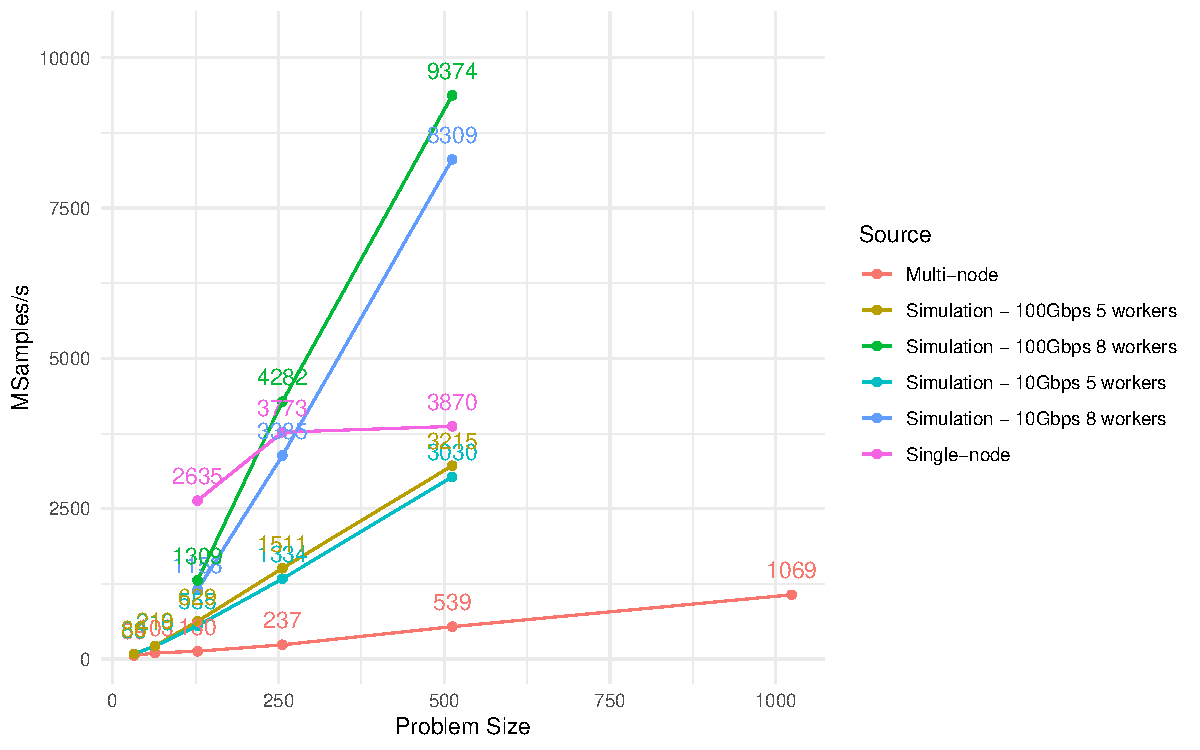
\includegraphics[width=\textwidth]{./assets/msamples.pdf}
\end{figure}

The most striking observation is the dramatic gap between 5-worker and
8-worker configurations. At $512^3$, the 8-worker simulations reach
8\,309~MSamples/s (10~Gbps) and 9\,374~MSamples/s (100~Gbps), while
the corresponding 5-worker results plateau at 3\,030 and
3\,215~MSamples/s---values that are below the
single-node baseline of 3\,870~MSamples/s. In other words, with 5
workers the communication overhead is so severe that distributing the
computation yields \emph{negative} speedup.

The root cause lies in the partitioning shape imposed by
\lstinline{MPI_Dims_create}. Since 5 is prime, it is forced into a
$\{5, 1, 1\}$ slices decomposition, whereas 8 factors into a
$\{2, 2, 2\}$ blocks decomposition. As established in
Section~\ref{sec:ghost_cells} and
Figure~\ref{fig:comms_vs_partitioning}, the total communication
boundary for slices grows as $2(P - 1)L^2$, while for blocks it grows
as $6(\sqrt[3]{P} - 1)L^2$. Concretely, for a $512^3$ domain with a
stencil thickness of 4 cells:

\begin{itemize}
  \item \textbf{5 workers $\{5,1,1\}$}: each slab measures
    $\approx 108 \times 512 \times 512$ and
    communicates with at most 2 neighbors, since the 1D partitioning
    produces no diagonal adjacencies. Each face halo is $4 \times
    512 \times 512 = 1\,048\,576$ doubles ($\approx 8$~MB). With two
    fields ($P$ and $Q$) and up to two neighbors, the total
    communication per iteration reaches $\approx 64$~MB.
  \item \textbf{8 workers $\{2,2,2\}$}: each sub-cube measures
    $260 \times 260 \times 260$ (including ghost cells) and
    communicates with 7 neighbors---3 on the same level and 4 on the
    adjacent level, including diagonal adjacencies. The face halos
    are $4 \times 256 \times 256 = 262\,144$ doubles ($\approx 2$~MB)
    each, while edge and corner halos are substantially smaller
    ($4 \times 4 \times 256$ and $4 \times 4 \times 4$, respectively).
    The total communication per iteration amounts to $\approx 25$~MB.
\end{itemize}

The block decomposition therefore reduces the per-worker communication
volume by approximately $2.5\times$, from 64~MB to 25~MB, despite
each worker communicating with more neighbors (7 vs.\ 2).

As expected from a balanced partitioning, the computation time
decreases proportionally when moving from 5 to 8 workers: at $512^3$
on the 100~Gbps simulated network, total computation drops from
$\approx 28$~s to $\approx 14$~s---consistent with the $8/5 = 1.6$
factor in available parallelism. This scaling of the computational
component is the expected behavior of a distributed implementation.

The MPI overhead, however, exhibits a disproportionately large
reduction that cannot be explained by the $2.5\times$ communication
volume difference alone. Furthermore, increasing the network bandwidth
tenfold (10~Gbps $\to$ 100~Gbps) barely improves the 5-worker
throughput (3\,030 $\to$ 3\,215~MSamples/s, $+6\%$), indicating that
the bottleneck in the $\{5,1,1\}$ configuration is not the network
bandwidth itself. The precise cause of this behavior remains to be
fully characterized through detailed profiling; however, it is
hypothesized that the large face size of the $\{5,1,1\}$ slabs
($512 \times 512$ per face, $\approx 8$~MB per halo) triggers
higher-latency MPI protocol paths (such as the rendezvous protocol
for large messages) and amplifies fixed per-transfer costs (PCIe
host--device copies, synchronization handshakes) that are independent
of network bandwidth and accumulate over the 1\,001 iterations of
the simulation.

Table~\ref{tab:results_summary} consolidates the approximate compute
load observed across all experimental scenarios, allowing a direct
comparison of the influence of backend, problem size and network
bandwidth on the masking effectiveness.

\begin{table}[H]
  \centering
  \caption{Summary of approximate compute load across all
  experimental scenarios.}
  \label{tab:results_summary}
  \begin{tabular}{llll}
    \hline
    Backend & Problem size & Network & Compute load \\
    \hline
    CPU (OpenMP) & $256^3$ & 10~Gbps (real)        & $\approx 75\%$    \\
    CPU (OpenMP) & $512^3$ & 10~Gbps (real)        & $\approx 87\%$    \\
    GPU (CUDA)   & $128^3$ & 1~Gbps (real)         & $\approx 20$--$25\%$ \\
    GPU (CUDA)   & $256^3$ & 1~Gbps (real)         & $\approx 20\%$    \\
    GPU (CUDA)   & $512^3$ & 1~Gbps (real)         & $\approx 20\%$    \\
    GPU (CUDA)   & $256^3$ & 10~Gbps (simulated)   & $\approx 65$--$70\%$ \\
    GPU (CUDA)   & $512^3$ & 10~Gbps (simulated)   & $\approx 75$--$80\%$ \\
    GPU (CUDA)   & $256^3$ & 100~Gbps (simulated)  & $\approx 85$--$90\%$ \\
    GPU (CUDA)   & $512^3$ & 100~Gbps (simulated)  & $> 90\%$          \\
    \hline
  \end{tabular}
\end{table}

\chapter{Conclusion}
\label{ch:conclusion}
The present research conceived a multi-node MPI implementation of
the Fletcher application with 3D block decomposition, asynchronous
ghost cell communication and GPU acceleration via CUDA, complemented
by a calibrated SimGrid simulation framework for exploring platform
configurations beyond those physically available.

The performance analyses emphasize the need for significant problem
domains, as well as high-speed network bandwidths to make up for the
MPI operations introduced. On the CPU backend (OpenMP) over the
10~Gbps \textit{cei} cluster, the compute load reached $\approx
75\%$ at $256^3$ and $\approx 87\%$ at $512^3$, demonstrating
effective masking already with general-purpose processors. On the GPU
backend (CUDA) over the 1~Gbps \textit{poti} cluster, however, the
compute load stagnated at $\approx 20\%$ regardless of problem
size, confirming that the Gigabit network is the predominant
bottleneck when paired with RTX~4070 accelerators. Simulated
scenarios revealed a clear progression: at 10~Gbps the compute load
rose to $\approx 65$--$80\%$, and at 100~Gbps it exceeded $90\%$,
confirming that the masking of communications, performed through
the use of overlapping computation with asynchronous calls, is
effective when the network bandwidth matches the computational
throughput of the accelerators. Furthermore, the 8-worker
$\{2,2,2\}$ block decomposition reached 9\,374~MSamples/s at
$512^3$ on the 100~Gbps simulated network, while the 5-worker
$\{5,1,1\}$ slices decomposition remained below the single-node
baseline, demonstrating the significant MSamples/s gains observed
under strict calibrated simulation.

The importance of proper domain segmentation is thereby proven for
this goal, as noted by the highlighted differences in the shapes
caused by the number of workers: prime process counts force a slices
partitioning that maximizes the boundary-to-volume ratio, nullifying
the benefits of distribution regardless of network capacity.
Combined with the inherent $O(n^2)$ boundary growth versus $O(n^3)$
volume growth, these results establish that both the partitioning
topology and the interconnection network are decisive factors for
the scalability of the distributed Fletcher with Ghost Cells application.

\section{Future work}
The results presented in the MPI implementation with ghost cells open a
set of promising directions for future investigations.

First, it is imperative to have
a more thorough analysis of the MegaSamples/second obtained with the
solution in scenarios where there is an adequate balance between the
interconnection network capacity and the computational capacity of the
accelerators, in order to precisely characterize the factors that are the
most influential in obtaining adequate results.

Second, experiments on the Santos Dumont supercomputer, especially on
partitions that allow the use of multiple GPU accelerators per node
with multiple MPI processes per node, are essential to evaluate the
behavior of the solution on a high-performance production platform with
a high-speed interconnection network, where the potential for masking
communication with computation can be fully exploited.

Third, the detailed modeling of the Santos Dumont interconnection
network in SimGrid SMPI would allow conducting local simulated
experiments with greater fidelity to the real environment, enabling the
evaluation of scale scenarios without the need for continuous access to
the machine and capacity planning tests for decision-making on the
pertinence of larger machines.

Finally, the integration of other computational kernels from other
accelerator programming APIs, such as HIP for AMD GPUs, would pave the
way for evaluating the relationship between kernel improvements
targeted at specific parallel accelerator architectures and the load
balancing between MPI computational nodes, allowing an understanding of
the extent to which kernel performance gains influence---or are limited
by---the efficiency of distributed communication.

\bibliographystyle{abntex2-alf}
\bibliography{./references.bib}
\printglossary
\appendix
\chapter{MPI Cartesian topology creation}
\label{ap:mpi_cart_create}
The code below illustrates the creation of a Cartesian topology in MPI
at a high level.

\begin{lstlisting}[style=CStyle, caption={Domain initialization in MPI}]
#include <mpi.h>
#include <stdio.h>

int main(int argc, char** argv) {
    MPI_Init(&argc, &argv);

    int world_rank, world_size;
    MPI_Comm_rank(MPI_COMM_WORLD, &world_rank);
    MPI_Comm_size(MPI_COMM_WORLD, &world_size);

    // 1. Distribute the workers across the dimensions
    int dims[3] = {0, 0, 0};
    MPI_Dims_create(world_size, 3, dims);

    // 2. Create the Cartesian communicator
    int periods[3] = {0, 0, 0};
    MPI_Comm cart_comm;
    MPI_Cart_create(MPI_COMM_WORLD, 3, dims, periods, 0, &cart_comm);

    // 3. Fetch the current process' coordinates
    int my_coords[3];
    MPI_Cart_coords(cart_comm, world_rank, 3, my_coords);

    // 4. Find and store all neighbors (26 neighbors + the current process)
    int neighbors[27];
    for (int face_index = 0; face_index < 27; face_index++) {
        // Displacement in each axis
        int dz = face_index / 9;
        int dy = (face_index % 9) / 3;
        int dx = face_index % 3;

        // Offset the displacement to have 0 equal the current process
        int neighbor_coords[3];
        neighbor_coords[0] = my_coords[0] + (dx - 1);
        neighbor_coords[1] = my_coords[1] + (dy - 1);
        neighbor_coords[2] = my_coords[2] + (dz - 1);

        // Fetch the neighbour's rank. If there is none, returns MPI_PROC_NULL
        MPI_Cart_rank(cart_comm, neighbor_coords, &neighbors[face_index]);
    }

    // 5. Send the forward neighbour a message
    int target_neighbor = neighbors[14];
    int buffer_send = 123;
    int buffer_recv = 0;
    MPI_Request reqs[2];

    if (target_neighbor != MPI_PROC_NULL) {
        printf("Rank %d sending a message to rank %d...\n", world_rank, target_neighbor);
        MPI_Isend(&buffer_send, 1, MPI_INT, target_neighbor, 0, cart_comm, &reqs[0]);
    }

    MPI_Finalize();
    return 0;
}
\end{lstlisting}

\chapter{Process initialization}
The pseudocode below illustrates how each process is initialized at a
high level.

\begin{lstlisting}[style=CStyle, caption = {Worker initialization}]
void worker_init() {
  partitions_data data;
  if(is_coordinator) {
    partitions_data partitions = coordinator_partition_cube();
    send_to_workers(partitions);
    data = fetch_coordinator_partition(partitions);
  } else {
    data = receive_from_coordinator();
  }
  anisotropy_vars anisotropy = compute_anistropy_variables();
  precomp_vars precomputation = compute_precomp_vars(anisotropy);

  worker_process(data);
}
\end{lstlisting}

\chapter{SimGrid computation sampling}
\label{ap:sampled_comp}
The C code below presents the algorithm behind the
sampling of the core computation of the program.

\begin{lstlisting}[style=CStyle, caption={Sampling and convergence mechanism for computation in SimGrid}, label={lst:sampled_comp}]
void sampled_computation(double *average, int *count, bool *converged,
                         void (*computation)(...)) {
    const double threshold = 0.05; // 5% error margin
    const int min_samples = 10;    // Minimum of samples for stability

    // If convergence has already been attained, we can just
    // simulate the workload
    if (*converged) {
        smpi_execute_benched(*average / 1e6); // Simulate time in SimGrid
        return;
    }

    // Measure real execution time
    double start = get_time_micros();
    computation(process, device_data); // Run actual kernel
    double end = get_time_micros();

    double current_val = end - start;

    // Update the average
    if (*average == -1) {
        *average = current_val;
    } else {
        *average = (*average * *count + current_val) / (*count + 1);
    }
    (*count)++;

    // Verify statistical stability convergence
    bool has_min_samples = (*count >= min_samples);
    bool is_stable = (fabs(*average - current_val) / *average) < threshold;

    if (has_min_samples && is_stable) {
        *converged = true;
    }
}
\end{lstlisting}

\end{document}
